\chapter{Mrežna aplikacija}
\label{chap:server}

Korisničko sučelje Orthobalancera ostvareno je kao mrežna aplikacija
implementirana također u Pythonu koristeći Flask microframework. Flask je
izgrađen na Werkzeug WSGI\footnote{Web Server Gateway Interface\cite{pep333}}
mrežnom alatu i Jinja2 sustavu predložaka. Flask je zvan \emph{microframeworkom}
jer svoju jezgru drži jednostavnom, ali proširivom. Flask također nudi određene
konvencije koje pojednostavljuju izgradnju mrežne aplikacije. Osim Flaska, za
razvoj aplikacije korišten je javascript uz većinu koda napisanu pomoću
biblioteke jQuery. Osim za asinkronu komunikaciju s poslužiteljem pomoću
AJAX-a\footnote{Asynchronous JavaScript and XML}, javasvript se najviše koristio
za postizanje dinamike te robusnosti provjere i sinkronizacije ulaznih podataka.

% pomalo o svakom bitnom url-u / templatu
HTML\footnote{HyperText Markup Language} stranice koje aplikacija generira
bazirane su na Jinja2 predlošcima. Jedno od njihovih pogodnih svojstava je
nasljeđivanje predložaka. Time se omogućuje da postoji jedan temeljni predložak
koji sadrži osnovne elemente svake stranice, a ostali samo nasljeđuju te
elemente i popunjavaju potrebni sadržaj. HTML predlošci Orthobalancera su
sljedeći:

\begin{itemize}

    \item \emph{layout.html} definira raspored svih elemenata te ga svi ostali
predlošci nasljeđuju.

    \item \emph{input.html} prihvaća ulazne podatke od korisnika. Detaljniji
opis mogućnosti koje su ostvarene za ulazne podatke se nalazi u odjeljku.
\ref{sec:input}

    \item \emph{manipulate\_exchangeable.html} je stranica koja se prikazuje
samo kada korisnik želi unijeti vlastite zamjenske čvorove taksonomskog stabla.
Stranica se otvara s ponuđenim pretpostavljenim skupom zamjenskih čvorova.

    \item \emph{execution.html}  prikazuje trenutno stanje izvođenja, asinkrono
komunicirajući sa poslužiteljem, kako bi korisnik imao jasniju predodžbu o
zadacima koje poslužitelj obavlja te o trajanju izvođenja. Jednom kada stranica
za ispis primi poruku o kraju izvođenja, automatski se preusmjerava na URL
\textbf{'/output'}.

    \item \emph{output.html} prikazuje izlaz aplikacije korisniku. Prikazani
izlaz je tablica na slici \ref{fig:tablica}. Osim tablice, nude se poveznice na
niz datoteka za preuzimanje. Izlazne datoteke su opisane u odjeljku
\ref{sec:output}.

    \item \emph{error.html} se prikazuje ukoliko na poslužitelju dođe do
pogreške.

\end{itemize}

Poslužitelj Orthobalancera se može zamisliti kao stroj stanja kojemu su stanja
predočena URL-om\footnote{unified resource locator}. Flask radi tako da veže
URL na jednu funkciju Pythona\footnote{\emph{view} funkcija} koristeći
mehanizam dekoriranja\cite{pep} funkcije kojeg nudi Python. Na taj se način uz
svaki URL veže određeni posao koji treba obaviti. Bitniji URL-ovi su sljedeći:

\begin{itemize}

    \item \textbf{'/'} ulazna točka za pokretanje novog upita. Upit dobiva
jedinstveni identifikacijski broj te se za njega inicijaliziraju određeni podaci
na poslužitelju kao sjednički podaci. Automatski se preusmjerava na
\textbf{/start}. Od ove točke na dalje svaki URL ima identifikacijski broj upita
u svome parametru, što nije posebno naznačeno. Takav je način prenošenja
identifikacijskog broja odabran kako bi korisnik samo pomoću URL-a mogao
dohvatiti svoje rezultate.

    \item \textbf{'/start'} pozvan za inicijalizirani upit. Generira i vraća
HTML stranicu baziranu na predlošku \emph{input.html}.

    \item \textbf{'/finish\_input'} poziva se tek u trenutku kad su na klijentskoj
strani svi ulazni podaci pravilno uneseni. Podaci su tada već spremljeni u
sjedničkim varijablama te se može stvoriti instanca razreda \emph{Pipeline},
odnosno nova dretva cjevovoda. Ovisno o korisnikovom odabiru na stranici
\emph{input.html}, sljedeće stanje izvođenja može biti na URL-u
\textbf{'/get\_exchangeable'} ako korisnik želi zadati svoje zamjenske čvorove,
odnosno na URL-u \textbf{'/preparations'} za pokretanje cjevovoda s predloženim
zamjenskim čvorovima.

    \item \textbf{'/preparations'} čita sadržaj datoteke sa predloženim
zamjenskim čvorovima, sprema ih u argumente sjednice te se preusmjerava na URL
\textbf{'/executing'}.

    \item \textbf{'/get\_exchangeable'} generira stranicu baziranu na predlošku
\emph{manipulate\_exchangeable.html} s podacima  iz datoteke s predloženim
zamjenskim čvorovima.

    \item \textbf{'/save\_exchangeable'} sprema korisnikove zamjenske čvorove u
argumente sjednice te se preusmjerava na URL \textbf{'/executing'}.

    \item \textbf{'/executing'} pokreće rad dretve cjevovoda te generira
stranicu baziranu na predlošku \emph{execution.html}.

    \item \textbf{'/output'} generira stranicu iz predloška \emph{output.html}
predajući joj sve potrebne informacije dohvaćene iz datoteka koje je stvorio
izlaz cjevovoda.

\end{itemize}

% TODO možda neki opis job/session (pitat Mile/Ivanu)
    
% LOG - možda posebna sekcija - TODO pitat
Vrijeme izvođenja posla u cjevovodu može potrajati nekoliko minuta te je zato
bilo potrebno osmisliti način kako predočiti korisniku napredak izvođenja u
nekom trenutku. Rješenje je osmišljeno na način da cjevovod svoj napredak
zapisuje u \emph{log} datoteke, a klijent asinkrono traži od poslužitelja
sadržaj tih datoteka svakih nekoliko sekundi. Za odvajanje funkcionalnosti
ispisa stanja cjevovoda u \emph{log} datoteke iskorišten je Pythonov mehanizam
dekoriranja funkcija. Implementirani su razredi \emph{beforeMessage} i
\emph{afterMessage} koji imaju funkcionalnost dekoratora. Oba dekoratora imaju
argument --- ključ rječnika koji sadrži konkretan tekst za ispis u \emph{log}
datoteke. \emph{beforeMessage} dekorira funkciju tako da obavlja ispis prije
poziva dekorirane funkcije, a \emph{afterMessage} nakon izvršavanja dekorirane
funkcije. Oba razreda dekoratora nasljeđuju temeljni dekorator
\emph{messagingDecorators} koji sadrži implementaciju samog zapisivanja statusa
u \emph{log} datoteke, a izvedeni razredi se samo brinu o načinu dekoriranja.

% TODO upute u sidebaru (možda nije potrebno - pitat)


\section{sinkronizacija ulaza}
\label{sec:input}

%ideja i srž implementacije sinkronizacije i ROBUSNOSTI unosa podataka slika

Jedan od nužnih preduvjeta za uspješan rad aplikacije jest pažljivo preuzimanje
ulaznih podataka uz robusne provjere. S druge strane bitno je omogućiti
raznolike načine unošenja podataka za lakše rukovanje aplikacijom. Orthobalancer
na ulazu očekuje dvije ili više proteinskih sekvenci od kojih će svaka
sadržavati različito ime. Elemente za unos podataka pojedinog proteina na
stranici moguće je dodavati dinamički. Sam FASTA zapis se može izravno upisati u
površinu za unos teksta, ili se može predati datoteka sa sadržajem FASTA zapisa.

Inicijalna ideja bila je sve provjere implementirati na strani klijenta pomoću
javascripta, no budući da javascript nije pogodan za otvaranje i čitanje
sadržaja datoteka odlučeno je da se podaci čuvaju na poslužitelju. Zbog toga je
potrebno prilikom svake promjene sadržaja bilo kojeg elementa unosa na stranici
sinkronizirati podatke sačuvane u sjedničkim varijablama na poslužitelju sa
trenutnim stanjem na stranici koju gleda korisnik. Sinkronizacije se događaju u
pozadini asinkronim komuniciranjem klijenta i poslužitelja. Asinkrona
komunikacija ostvarena je AJAX tehnologijom, a klijent i poslužitelj prenose
podatke u JSON\footnote{JavaScript Object Notation} formatu, za što Flask ima
kvalitetnu podršku.

\begin{figure}[h!]
\centering
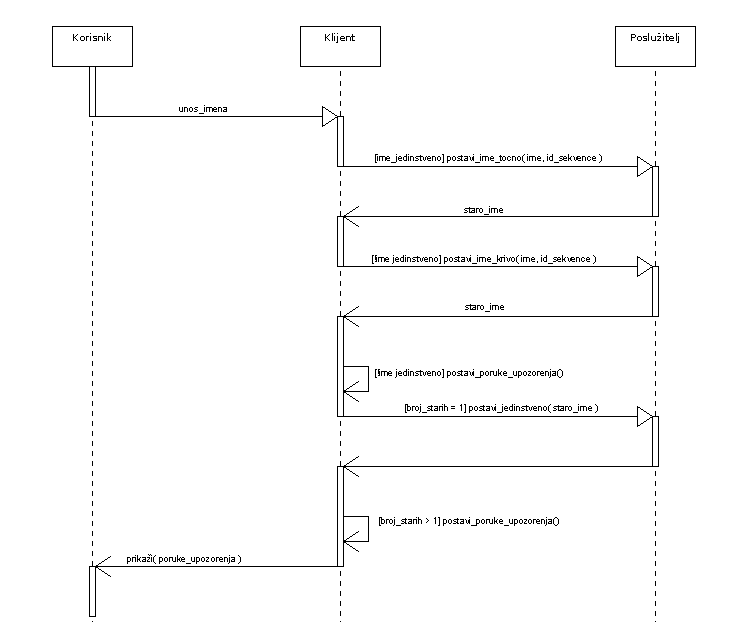
\includegraphics[width=6.1in, height=6in]{figures/Unos_imena.png}
\caption{UML sekvencijski dijagram koji prikazuje slijed operacija prilikom
unosa imena}
\label{fig:imena}
\end{figure}

% UNOS IMENA
Obrada i spremanje podataka prilikom unosa imena sekvence prikazani su
UML\footnote{Unified Modeling Language} sekvencijskim dijagramom na slici
\ref{fig:imena}. Obrada počinje automatski u pozadini netom nakon što se ime
unese. Klijent najprije pretražuje imena svih vidljivih sekvenci. Ukoliko je
postavljeno ime različito od svih drugih unesenih imena, AJAX pozivom se
dojavljuje poslužitelju da postavi uneseno ime za tu sekvencu. Nakon što postavi
ime, poslužitelj provjerava validnost svih podataka za danu sekvencu te vraća
staro ime koje je bilo pridruženo sekvenci. Klijent briše eventualne poruke
upozorenja za danu sekvencu jer je ime jedinstveno. U slučaju da uneseno ime
nije jedinstveno, AJAX-om se dojavljuje poslužitelju uneseno ime uz naznaku da
je krivo. Svim sekvencama sa unesenim imenom poslužitelj miče zastavicu da su
jedinstvena te pokreće validciju njihovih podataka. Poslužitelj opet vraća staro
ime sekvence sa promijenjenim imenom. Također, u slučaju nejedinstvenog unesenog
imena, svim HTML elementima s istim imenom se pridružuje prikladna poruka
upozorenja. Nakon postavljanja imena na poslužitelju, klijent je dužan
provjeriti jesu li neka od jednakih imena na stranici trenutnim unosom
razriješena. Klijent dohvaća sve elemente s imenom jednakim starim imenom koje
je poslužitelj vratio. Ukoliko takvih nema, ništa se ne događa jer problema niti
nije bilo. Ako ih je više, na primjer 2, to znači da ih je prethodno bilo 3, ali
ta se imena i dalje trebaju razriješiti tako da im se poruke upozorenja ne miču.
Na poslijetku, ako je samo jedno ime pronađeno, njemu se brišu poruke upozorenja
te se AJAX-om dojavljuje poslužitelju da je ono od sada jedinstveno. Poslužitelj
označava ime jedinstvenim te pokreće validaciju nad tom sekvencom.

Unos sekvence korisnik može obaviti na dva načina: može napisati ili zalijepiti
FASTA sekvencu u područje za unos teksta ili može \emph{uploadati} FASTA
datoteku. Ako je odabran tekstualni način, jednom kada se sekvenca upiše u
površinu za unos aktivira se logika koja predaje sekvencu poslužitelju na obradu
AJAX pozivom. Za slučaj kada je odabran \emph{upload} FASTA datoteke ne može se
koristiti AJAX. AJAX tehnologija je u mogućnosti slati samo čisti tekst, a
javascript nije u mogućnosti otvarati datoteke odabrane za \emph{upload}. Iz tih
razloga se ovdje koristi pomalo zastarjelo i ne sasvim pouzdano, ali jedino
preostalo rješenje, a to je simuliranje \emph{submita} HTML forme i korištenje
HTML \emph{iframe} taga. \emph{iframe} tag u svojoj osnovnoj funkcionalnosti
omogućava prikaz bilo koje druge stranice unutar osnovne stranice koju je
korisnik zatražio, drugim riječima \emph{iframe} element je kao prozor koji
prikazuje neku drugu stranicu. No ako \emph{form} tagu koji sadrži sve elemente
ulaznih podataka za \emph{target} tag postavimo ime \emph{iframea} na istoj
stranici, sadržaj trenutne stranice ostati će nepromijenjen, što uključuje i sve
podatke u \emph{input} elementima koje je korisnik unio. U ovome slučaju, gdje
je potrebno asinkrono prenijeti datoteku do poslužitelja, dodane su sljedeće
akcije. Prilikom odabira datoteke za \emph{upload} automatski se poziva
javascript fukcija koja simulira \emph{submit} glavne forme. Poslužitelj potom
preuzima datoteku, sprema ju, poziva obradu sekvence i vraća tijelo javascript
poziva kojim se označava kraj slanja datoteke poslužitelju. Minimalni uvjet koji
sama datoteka mora zadovoljiti jest da ima nastavak \emph{.fasta} ili
\emph{.txt}.

Obrada sekvence na poslužitelju prvenstveno provjerava jesu li predani podaci
doista u FASTA formatu. Zapis ne mora nužno sadržavati FASTA zaglavlje jer
korisnik može upisati ime koje želi, a ime je jedino što bi se uzimalo iz
zaglavlja ulaznih sekvenci. Za sekvencu je bitno da ne sadrži nedozvoljene
znakove koji ne predstavljaju niti jednu aminokiselinu. Sekvenca se za daljnju
obradu sprema u varijable sjednice kao jedan znakovni niz velikih slova bez
bjelina. Na kraju obrade pokreće se validacija nad tom sekvencom.

% BRISANJE PROTEINA SA STRANICE
Sekvence na stranici moguće je dinamički dodavati i brisati. Dodavanje nove
sekvence samo umeće nove HTML elemente na stranicu, a podaci za tu sekvencu se
inicijaliziraju na poslužitelju prilikom prvog AJAX poziva koji sadrži tu
sekvencu. Brisanje sekvence zahtijeva određene akcije. Klijent najprije sakrije
obrisanu sekvencu, iako ona još uvijek posoji. Zatim pretraži i dohvati sve
elemente s imenom jednakim imenu obrisane sekvence. Nakon toga, klijent AJAX
pozivom dojavljuje poslužitelju da je određena sekvenca obrisana, prosljeđujući
mu istovremeno niz istoimenih sekvenci. Poslužitelj označava obrisanu sekvencu
neaktivnom i pokreće validaciju nad njome. Na kraju, ako je duljina niza
istoimenih elemenata jednaka 2, to znači da od trenutka brisanja drugi element
ima jedinstveno ime. Poslužitelj označava ime druge sekvence jedinstvenim te
pokreće validaciju nad njome. Po povratku na klijenta, ako je duljina niza bila
jednaka 2, miču se poruke upozorenja druge sekvence.

% VALIDACIJA    # check_ok()
Validacija pojedine sekvence na poslužitelju postoji kako bi se svi podaci dane
sekvence provjerili jesu li uneseni i jesu li u dozvoljenom obliku kako bi se
jednostavnom provjerom zastavice 'OK' moglo ustvrditi može li dana sekvenca biti
proslijeđena u cjevovod. Prilikom validacije događaju se sljedeće provjere:

\begin{itemize}

\item je li sekvenca još aktivna?

\item je li uneseno ime jedinstveno? Ako nije, iznimno dozvoli za slučaj u kojem
ime nije uneseno, a postoji ime u FASTA zaglavlju unesene sekvence.

\item je li unesena sekvenca?

\end{itemize}

Jednom kad korisnik pritisne bilo koju od tipki za nastavak, bilo da je to
\emph{Proceed} ili \emph{Modify exchangeable nodes}, pretpostavlja se da su svi
podaci već spremljeni na poslužitelju. Pritiskom na tipku pozvat će se
\emph{submit} alternativne forme koja je vezana za provjeru validnosti podataka.
Forma je također vezana za svoj \emph{iframe} za slučaj da svi podaci nisu
spremni za pokretanje cjevovoda. \emph{iframe} je ovdje potreban kako se ne bi
izgubili svi podaci koje je korisnik unio.  Poslužitelj ovdje samo provjerava
izračunatu validnost podataka te vraća tijelo javascript poziva kojim se
ispisuje ispravna poruka o grešci ili kojim se izvodi \emph{submit} konačne
forme za nastavak izvođenja.

% TODO treba li opisati i manage exchangeable?
